%        File: proposal.tex Created: Wed Nov 07 07:00 PM 2018 E Last Change: Wed
%     Nov 07 07:00 PM 2018 E
%
\documentclass[letterpaper, 12pt]{article}
\usepackage{bbm}
% \usepackage{hyperref
\usepackage[thm]{macros}
% \usepackage{natbib}
% \usepackage{nopageno}
\newgeometry{margin=1in}
\usepackage{lipsum}
\pagestyle{fancy}
\lhead{}
\chead{\textsc{High-dimensional GLMs}}
\rhead{}

\newcommand{\by}{\bm y}
\newcommand{\bx}{\bm x}
\newcommand{\bX}{\bm X}
\newcommand{\bW}{\bm W}
\newcommand{\stb}{\bm e}
\newcommand{\bbeta}{\bm \beta}
\newcommand{\one}{\mathbbm{1}}
\newcommand{\trans}{\intercal}
\newcommand{\bg}{\bm g}
\newcommand{\bgamma}{\bm \gamma}
\newcommand{\linearlasso}{\hat \bbeta_{\text{lasso}}}
\newcommand{\linearlassofitted}{\hat \by_{\text{lasso}}}
\newcommand{\empave}{\mathbf{P}_n}
\newcommand{\theoave}{\mathbf{P}}
\newcommand{\bZ}{\bm Z}
\newcommand{\err}{\mathcal{E}}

\begin{document}

\title{\textbf{Model Selection and Estimation in High-dimensional
Generalized Linear Models}}
\author{\textbf{Francisco Rivera} \\ Harvard College \and \textbf{Jiafeng (Kevin) Chen} \\ Harvard College}
\date{\today}

\maketitle
\doublespacing
\section{Introduction}
\label{sec:intro}
High-dimensional statistics---settings in which the dimensionality of the
predictors, $p$, is high, or even higher than that of the data $n$---has become
increasingly prevalent. Typically in such settings, we assume that the
underlying signal is \emph{sparse}---only $k$ of the $p$ predictors, $k \ll p$,
are actually predicative.\footnote{``Use a procedure that does well in sparse
problems, since no procedure does well in dense problems'' 
\citep{hastie2015statistical}.} Traditional methods, like ordinary least squares
or maximum likelihood, typically do not work well in high-dimensional settings
as we cannot impose sparsity without model selection; moreover, model selection
is an
optimization problem of the prohibitive dimension $2^p$, and greedy methods such
as forward/backward stepwise selection are typically ad hoc. 

The workhorse for high-dimensional regressions is the $\ell_1$ lasso penalty
\citep{tibshirani1996regression}. In this report, we focus on properties of
the lasso. The original lasso is developed for fitting
(normal) linear models with the objective\footnote{We consider $\by$ an
$n$-vector of response variables whose $i$th element is $\by_i$. We consider the
covariate matrix $\bX$ ($n \times p$). In most settings, $\bX$ include an
intercept column, $\bx_{0} = \bm 1$, that is not regularized.} \begin{equation}
    \hat \bbeta_{\text{lasso}} = \argmin_{\bbeta}\, \frac{1}{2n}\norm{\by -
    \bX\bbeta}^2 + \lambda \norm{\bbeta}_1 - \lambda |\beta_0|, \, \lambda > 0.
    \label{eq:linear_lasso}
\end{equation}
The first paper about lasso in a GLM setting is \cite{park2007l1}: Consider a scalar GLM with likelihood \[
L(y; \theta,\phi) = \exp\br{\frac{y\theta - b(\theta)}{a(\phi)} + c(y, \phi)},
\]
where $g(\E[y]) = \eta = \bx^\trans \bbeta$ for some scalar function $g$. Thus
we may consider a direct extension of \eqref{eq:linear_lasso}: \begin{equation}
    \hat \bbeta_{\text{GLM-lasso}} = \argmin_{\bbeta}\,
    \underbrace{-\frac{1}{n}\sum_{i=1}^n \bk{y_i \theta(\bbeta)_i -
    b\pr{\theta(\bbeta)_i}}}_{\ell_n(\bbeta)} + \lambda \norm{\bbeta}_1 -
    \lambda |\beta_0|,
    \label{eq:glm_lasso}
\end{equation}
where \eqref{eq:glm_lasso} reduces to \eqref{eq:linear_lasso} if the likelihood
is Gaussian and $g$ is the canonical link for the Gaussian model, which is the
identity function. Note that the objective \eqref{eq:glm_lasso} is convex if we
use the canonical link, since the exponential family log-likelihood is concave
in $\theta$, and $\theta = \bx^\trans \bbeta$ is linear in $\bbeta$ for the
canonical link.

This report is organized as follows. \Cref{sec:model} discusses theoretical
properties with respect to the in-sample error $\E\pr{\E[y \mid \bx] - \hat f
(\bx)}^2$ and selection error for the lasso with linear and generalized linear
models. \Cref{sec:estimation} discusses algorithmic properties of lasso
estimation, primarily in a generalized linear model context, as the linear lasso
estimation problem is well understood \citep{efron2004least}. \Cref{sec:num}
illustrates the lasso with numerical simulations. \Cref{sec:conc} concludes.

\section{Model Selection with Lasso}
\label{sec:model}

Brute-force model selection scales poorly with respect to the number of
predictors. That is, when building a model to predict $\bm{y}$ from a subset of
the columns of $\bX \in \mathbb{R}^{n,p}$ (since not all columns may be
predictive), there are $2^p$ subsets of columns to regress on. Checking all of
these models against each other incurs a cost exponential in $p$ and becomes
prohibitively expensive in a high-dimensional setting. In class, we tackled this problem with forward-selection and backward-deletion,
a greedy algorithm that adds and removes covariates until a local optimal is
reached. 

We introduced the lasso \eqref{eq:linear_lasso} in \Cref{sec:intro}. We first
summarize the literature on lasso with OLS in
this section. Assume that $\by = \bX \bbeta^\star + \bm \epsilon,\, \bm\epsilon
\sim
\Norm(0, \sigma^2 \bm I_n)$. In this case, where possibly $p > n$, the OLS
estimate $\hat \bbeta
\in \argmin_{\bbeta} \norm{\by - \bX \bbeta}^2$ may not be unique, but all such
solutions have the same fitted values $\hat \by_{\text{OLS}} = \bX \hat\bbeta$.
\begin{prop}
    For some constant $C$, with $r = \text{rank}(\bX)$, then $
    \E\bk{
    \norm{X\bbeta^\star - \hat \by_{\text{OLS}}}_2^2 
    } \le Cr\sigma^2.
    $
\label{thm:ols_bound}
\end{prop} 
\begin{proof}
    Observe that \begin{align*}
\norm{\by - \hat \by}^2  = \norm{\bX \bbeta^\star - \bX\bbeta} + 
\norm{\bm \epsilon}_2^2 + 2 \bm \epsilon^\trans \pr{\bX \bbeta^\star -
\bX\bbeta},
\end{align*}
for any $\bbeta$. Note that $\norm{\by - \hat \by_{\text{OLS}}}^2 \le \norm{\bm
\epsilon}_2^2$. Thus \begin{align*}
\norm{\by - \hat \by_{\text{OLS}}}^2  &= \norm{\bX \bbeta^\star - \hat \by_{\text{OLS}}} + 
\norm{\bm \epsilon}_2^2 + 2 \bm \epsilon^\trans \pr{\bX \bbeta^\star - \hat \by_{\text{OLS}}} \le \norm{\bm
\epsilon}_2^2\\
\implies \norm{\bX \bbeta^\star - \hat \by_{\text{OLS}}} &\le
2\bm\epsilon^\trans\underbrace{\pr{\hat \by_{\text{OLS}} - \bX \bbeta^\star}}_
{\in C(\bX)}.
\end{align*}
Thus we can write $\hat \by_{\text{OLS}} - \bX \bbeta^\star = \bm \Phi \bm \nu$,
for some $n\times \text{rank}(\bX) =: n\times r$ matrix $\bm \Phi$ of
orthonormal basis of the columns of $\bX$. Thus \[
\frac{\bm\epsilon^\trans{\pr{\hat \by_{\text{OLS}} - \bX \bbeta^\star}}}{
\norm{\bX \bbeta^\star - \hat \by_{\text{OLS}}}} = \frac{\bm \epsilon^\trans
\bm \Phi \bm \nu}{ \norm{\bm \Phi \bm \nu}_2} = \pr{\bm\Phi^\trans\bm
\epsilon}^\trans \frac{\bm \nu}{ \norm{\bm\nu}} \le \sup_{\bm u : \norm{\bm u}
\le 1}  \pr{\bm\Phi^\trans\bm
\epsilon}^\trans u.
\]
Using the above inequalities, we show that \[
\norm{\bX\bbeta^\star - \hat \by_{\text{OLS}}}^2 \le 4 \pr{\sup_{\bm u, 
\norm{\bm u} \le 1}
\underbrace{(\bm\Phi^\trans \bm\epsilon )^\trans}_{\Norm(0, \sigma^2 \bm I_r)}
\bm u}^2 \implies \E\bk{\norm{\bX\bbeta^\star - \hat \by_{\text{OLS}}}^2} \le
4\sigma^2 r,
\]
by properties of the normal distribution.\end{proof}

Let $\linearlasso$ be the linear lasso estimate as in \eqref{eq:linear_lasso}.
Let $\linearlassofitted$ be its fitted value. We can show that a bound similar
to \Cref{thm:ols_bound} for the lasso, with $O_\P(\sqrt{\log (p/n)})$ replacing
the $O
(r/n)$ dependence (This is the so-called \emph{slow rate} for the lasso, see
\cite{tibshirani2015sparsity}). Using the fact that $\linearlasso$ must achieve
a better value than $\bbeta^\star$ for the objective in 
\eqref{eq:linear_lasso}, and an expansion similar to the one in the proof of
\Cref{thm:ols_bound}, we can show the inequality \begin{align*}
\frac{1}{2n} \norm{\bX \bbeta^* - \linearlassofitted}_2^2 &\le \frac{1}
{n}\underbrace{\bm
\epsilon^\trans \pr{\linearlassofitted - \bX \bbeta^*}}_{\le \norm{\bX^T
\bm\epsilon}_\infty \norm{\linearlasso - \bbeta^\star}_1 \text{(H\"older)}} +
\lambda \norm{\bbeta^
\star}_1 - \lambda \norm{\linearlasso}_1 \tag{\emph{Basic inequality} for the
lasso}.
\label{eq:basic} \\
&\le \lambda \pr{\norm{\linearlasso - \bbeta^\star}_1 + \norm{\bbeta^
\star}_1 - \norm{\linearlasso}_1 } \tag{On events $\Omega = \br{n^{-1}
\norm{\bX^T
\bm\epsilon}_\infty \le \lambda }$} \\
&\le 2\lambda \norm{\bbeta^\star}_1.
\end{align*}
We can show that $
\P(\Omega) \ge 1 - p^{-C/2 + 1}
$ if $\lambda = C\sigma \sqrt{\log (p) / n}$ for $C > 2$, assuming standardized
columns in $\bX$ \citep[see][]{tibshirani2015sparsity}. This leads to the
following 

\begin{prop}[Slow rate for the lasso]
    Let $\lambda =  C\sigma \sqrt{\log (p) / n}$ for $C > 2$, then with
    probability at least $1 - p^{-C/2+1}$, \[
    \frac{1}{n}\norm{\bX \bbeta^* - \linearlassofitted}^2 \le 2 
    \norm{\bbeta^\star}_1 \sigma \sqrt{C \frac{\log p}{n}}.
    \]
\end{prop}
How far is the lasso from the optimum? Suppose $k < p$ of $\bbeta^\star$ are
nonzero, then if we knew these active predictors (i.e. have an \emph{oracle}),
the
{oracle} OLS estimator achieves an error of
$k\sigma^2/n$. One can show that the error cannot get better than $\log(p)
k\sigma^2/n$ without the oracle, and the best-subset estimator---replacing
$\ell_1$-norm in \eqref{eq:linear_lasso} with the nonconvex $\ell_0$-norm, $\norm{\bbeta}_0 =
\sum_i
\one\pr{\bbeta_i \neq 0}$---achieves this optimum. Under certain conditions, we
can show that the lasso achieves a \emph{fast rate} of $\log(p) k\sigma^2/n$,
which is the optimal rate. \cite{van2009conditions} provide a review of relevant
conditions for achieving the fast rate. These conditions mostly forbid high
correlations among the active columns in $\bX$.\footnote{Roughly speaking,
such assumptions allow us to bound the difference in $\bbeta$ in terms
of the difference in fitted values. Since the difference in fitted values are
naturally bounded by differences in $\bbeta$, this allows us to recover an
independent bound on the difference of fitted values (in-sample error). See
\cite{tibshirani2015sparsity} for details.}
Moreover, with even more
restrictions, one could show that there exists a
$\lambda$ in
\eqref{eq:linear_lasso} for which the corresponding $\linearlasso$ achieves
perfect \emph{support recovery} with high probability: \[
\sgn(\linearlasso) = \sgn(\bbeta^\star).
\]
We defer the more technical discussions to \cite{buhlmann2011statistics}. 

Chapter 6 of \cite{buhlmann2011statistics} extends much of the linear results to
convex loss functions, covering scalar-valued GLMs with canonical links. Let
$\rho_{f_{\bbeta}}$ be a loss function with respect to prediction function
$f_\beta$ that maps data $\bm Z_i = (\bx_i, \by_i)$ to $\R$. Denote $\empave
\rho = n^{-1}\sum_i\rho(\bZ_i)$ the empirical risk, $\theoave \rho = n^{-1} \E
\bk{\sum_i \rho
(\bZ_i)}$ the theoretical risk, and $\err(f) = \theoave\pr{\rho_f - \rho_{f_0}}$
the excess risk,
where $f_0$ is a
minimizer of $\theoave \rho$ in some class $\mathbf{F} \supset \mathcal F = 
\{f_{\bbeta}: \bbeta \in \R^p\}$. Let $f^0_{\text{GLM}} = \argmin_{\mathcal F}
\theoave \rho$ be the GLM approximation to $f_0$, which is assumed to have low
excess risk. In the GLM context, let $\bbeta^\star$ be the parameters such that
$f_{\bbeta^\star} = f_{\text{GLM}}^0$. 
The lasso in this context produces \[
\hat \bbeta = \argmin_{\bbeta} \br{\empave \rho_{f_{\bbeta}} + \lambda 
\norm{\bbeta}_1 }.
\]
Define the \emph{empirical process} to be the gap between theoretical and
empirical risks for a $\bbeta$: $\br{v_n (\bbeta) = (\empave - \theoave)
\rho_{f_{\bbeta}}: \bbeta \in \R^p}$. The \eqref{eq:basic} can be generalized to
\[
\err\pr{f_{\hat \bbeta}} + \lambda \norm{\hat \bbeta}_1 \le -\pr{v_n (\hat
\bbeta) - v_n (\bbeta^\star)} + \lambda \norm{\bbeta^\star}_1 + \err\pr{f_
{\bbeta^\star}}
\]
Using the above, we show that, with probability that converges to 1 as $\lambda
\to 0$, \[
\err(f_{\hat \bbeta}) + \lambda \lVert\hat \bbeta \rVert_1 \le 2 \bk{
    \err(f_{\bbeta^\star}) + 2\lambda \norm{\bbeta^\star}_1
}  
\]
as $\lambda \to 0$, this shows a sort of \emph{consistency} result. For
instance, if the true $f$ is a GLM, then $\err(f_{\hat \bbeta}) \to 0 = 2
\err(f_{\bbeta^\star})$.  We can also show \cite[][Chapter 6.7]
{buhlmann2011statistics} an \emph{oracle inequality} similar to that in the fast
rate of the lasso, where under some restrictive regularity conditions, $\err(f_
{\hat \bbeta})$ shrinks at the oracle rate of $O\pr{k \log p / n}$. 

\section{Estimation}
\label{sec:estimation}

\subsection{Regularization path methods}
\cite{efron2004least} gives an efficient estimation procedure for the linear
lasso \eqref{eq:linear_lasso} called the Least Angle Regression (LAR), which
relies on the fact that the \emph{regularization path}---$\hat \bbeta_i$ as a
function of $\lambda$---is piecewise linear in \eqref{eq:linear_lasso}. Such a
structure is often unavailable in applications like \eqref{eq:glm_lasso}. \cite{park2007l1} mimicks the LAR procedure in GLM estimation. The high-level idea is to note the
non-zero coefficients for different penalizations $\lambda$ and constrain our
search to these models. We describe their procedure in this section.

In order to employ this method, we require a method to solve
\eqref{eq:glm_lasso}. For now, we suppose that we have such a method and can use
it as a black box. It is sufficient for us to know that this black box takes in
an initial $\bbeta^\text{init}$ and employs a descent-based method to converge
toward the optimal $\bbeta^*$. \cref{sec:estimation} follows-up by describing
the inner workings of different approaches.

The lasso penalty induces a sparsity in our optimal $\bbeta$. This sparsity
increases as our penalization term $\lambda$ becomes bigger. Indeed, if we take
$\lambda \to \infty$, then our solution is driven to $\bbeta \to \bm{0}$ because
the penalization term is all that matters, and the norm of $\bbeta$ is minimized
at $\bm{0}$. The entire domain when $\bbeta = \bm{0}$ is uninteresting, so we
initialize our algorithm at $\lambda_\text{max}$ which we define as the smallest
$\lambda$ such that there is only one non-zero coefficient.

Once we have initialize $\lambda$ in our algorithm to $\lambda_\text{max}$, we
will repeat three steps that \cite{park2007l1} outline,

\begin{enumerate}

\item Determine the step length by which to decrease $\lambda$. The intent is to
pick this such that the precisely one more coefficient becomes non-zero.
Introducing notation, we let $\lambda_k$ be the $\lambda$ value we consider in
the $k$th step, and we have to pick $\lambda_k - \lambda_{k+1}$.

\item Using a linear approximation, predict the value of $\bbeta$ for the
decremented $\lambda_{k+1}$.

\item Initialize our solver of \eqref{eq:glm_lasso} with the linear estimate as
$\bbeta^\text{init}$ and get the precise solution $\bbeta^*$ for the new
$\lambda$.

\end{enumerate}

doing so until either we have brought $\lambda$ all the way to 0, or we
determine that incremental variables are not improving the model. In order to
perform the second step, a linear approximation prescribes that,

\[ \bbeta_{k+1} \approx \bbeta_k + (\lambda_{k+1} - \lambda_k) \frac{\partial
\bbeta}{\partial \lambda}.\]

Denote by $\bX_A$ the matrix made up by the columns of $\bX$ whose corresponding
$\bbeta$ coefficient is non-zero, i.e. in the active set. Furthermore, let $\bW$
be the diagonal matrix with $i^\text{th}$ diagonal element given by,

\[ \frac{1}{\var(y_i)} \left( \frac{\partial \mu}{\partial \eta} \right)^2\]

which changes because the derivative is evaluated at a different location based
on the value of $\lambda$, so we define $\bW_k$ as the value of $\bW$
corresponding to $\lambda_k$. Then, we have that,

\[ \bbeta_{k+1} \approx \bbeta_k - (\lambda_{k+1} - \lambda_k) (\bW_A^\top \bW_k
\bX_A)^{-1} \sgn (\beta_k).\]

Note that in the above equation, we pretend $\bbeta_k$ and $\bbeta_{k+1}$ only
contain their non-zero components, and thus are not going to have all $p$
dimensions. This makes our algebra simpler and we can do this because the linear
approximation will not make a previously zero coefficient non-zero.

Finally, we just need to determine our step size. One simple choice could be to
use a constant step size. However, in different domains of $\lambda$, the same
unit change in $\lambda$ could have dramatically different implications for the
sparsity of the resulting $\bbeta$. If we were working with a lasso in linear
regression, $\bW$ would not change, and we could pick the step size precisely to
coincide with the point at which a coefficient of zero becomes non-zero.
\cite{park2007l1} suggest doing precisely this, with the caveat that because
$\bW$ does change, it will only be an approximation for the GLM case. 

\subsection{Coordinate descent methods}
Unfortunately, \cite{park2007l1}'s method often scales poorly with the size of the problem. The
most popular method---proposed by \cite{friedman2010regularization} and
implemented in \textsf{R}'s \textsf{glmnet} package---is \emph{cyclical
coordinate descent} with iteratively reweighted least squares. The idea is to
approximate $\ell_n(\bbeta)$ in \eqref{eq:glm_lasso} with a second-order Taylor
expansion, either globally for all parameters $\bbeta$ (for scalar-valued GLMs)
or locally with a single parameter $\bbeta_j$ (for vector-valued GLMs, such as
the multinomial logistic regression). Such an approximation yields a quadratic
function (in the scalar GLM case) \[
\ell_{Q}(\bbeta) = \frac{1}{n}\sum_{i=1}^n w_{i} (y_i - \bx_i^\trans \bbeta)^2.
\]
We then solve a local penalized least-squares problem:\begin{equation}
    \bbeta \gets \argmin_{\bbeta} \ell_{Q}(\bbeta) + \lambda \norm{\bbeta}_1.
    \label{eq:local_opt}
\end{equation}
via cyclical coordinate descent, i.e. by iteratively solving \begin{equation}
    \bbeta_j \gets \argmin_{\bbeta_j} \ell_{Q}(\bbeta) + \lambda \norm{\bbeta}_1,
    \label{eq:cyclic_opt}
\end{equation}
holding all other entries $\bbeta_{-j}$ fixed. \eqref{eq:cyclic_opt} has an analytical solution for the lasso penalty\footnote{\cite{friedman2010regularization} show a similar expression for the \emph{elastic net} penalty: \[
\lambda P_\alpha(\bbeta) = \lambda \pr{\alpha \norm{\bbeta}_1 + (1-\alpha) \norm{\bbeta}_2}.
\]}
\begin{equation}
    \bbeta_j \gets \frac{S\pr{\sum_{i=1}^N w_i x_{ij}\pr{y_i - \tilde y_i\uppr{j}}, \lambda}}{\sum_{i=1}^N w_i x_{ij}^2}, \, S(t, \gamma) = \sgn(t)\pr{|z|-\gamma}_+,\, \tilde y_i\uppr{j} = \bx_i^\trans \bbeta - x_{ij}\bbeta_j.
    \label{eq:ccd_update}
\end{equation}
We summarize the procedure described above in \Cref{alg:ccd}. 
\begin{algorithm}
\caption{Cyclic coordinate descent algorithm for solving \eqref{eq:glm_lasso} (scalar GLM case) in \cite{friedman2010regularization}}
\label{alg:ccd}
\begin{algorithmic}
\State{Initialize $\bbeta$}
\For{$\lambda$ on regularization path}
\While{$\bbeta$ has not converged}
\State{Approximate $\ell_n(\beta)$ by $\ell_Q(\beta)$}
\While{cyclical descent has not converged}
\For{$j$}
    \State{Update $\bbeta_j$ according to \eqref{eq:ccd_update}}
\EndFor
\EndWhile
\EndWhile
\State{$\hat{\bbeta}_\lambda \gets \bbeta$}
\State{Initialize $\bbeta$ for next iteration to $\hat{\bbeta}_\lambda$}
\EndFor
\end{algorithmic}
\end{algorithm}

The machine learning literature slightly alters \Cref{alg:ccd} and changes \eqref{eq:ccd_update} into \[
\bbeta_j \gets S\pr{\bbeta_j - \pr{\nabla_{\bbeta} \ell_n(\bbeta)}_j \kappa^{-1}, \frac{\lambda}{\kappa}}
\]
for some \emph{learning rate} $1/\kappa$, in keeping with gradient descent. Moreover, \cite{shalev2011stochastic} proves a convergence guarantee for stochastic coordinate descent in this fashion, where, instead of cycling through the coordinates of $\bbeta$, a coordinate is chosen uniformly at random. 
\begin{theorem}
Let $Q(\bbeta)$ be the objective in \eqref{eq:glm_lasso}. 
    At iteration $T$ of the first while-loop in a verison of \Cref{alg:ccd} with stochastic coordinate descent and gradient updates, \[
    \E[Q(\bbeta_T)] - \E[Q(\hat\bbeta_{\text{GLM-lasso}})] \le C\frac{p \kappa}{T+1}
    \]
    for constant $C$ a function of the initial starting value $\bbeta\uppr{0}$, assuming that $\ell_n$ is differentiable with \[
    \ell_n (\bbeta + \eta \stb_j) \le \ell_n(\bbeta) + \eta \pr{\nabla \ell_n}_j + \frac{\kappa}{2} \eta^2
    \]
    for all $\eta, \bbeta, j$.\footnote{This condition restricts the choice of $\kappa$ as a function of the loss criterion.}
\end{theorem}
\begin{cor}
    The runtime to achieve $\epsilon$ expected accuracy is bounded by \[O\pr{\frac{np\kappa }{\epsilon} \norm{\hat \bbeta_{\text{GLM-lasso}}}_2^2}.\]
\end{cor}

Moreover, \cite{bradley2011parallel} show that a parallel version of the
coordinate gradient descent procedure above where at each iteration, $\mathsf P$
(possibly duplicate) coordinates are updated in parallel. For correlated
features, such parallelism is dangerous, since updating two correlated features
simulataneously may over or undercompensate for the gradient direction.
\cite{bradley2011parallel} quantifies the interference due to correlated
features and shows that efficiency increases linearly in the number of parallel
processes $\mathsf{P}$ so long as $\mathsf{P} \le \frac{p}{\rho}$ where $\rho$
is the largest modulus of the eigenvalues of $X^\trans X$.

Coordinate descent methods described above can also become expensive if $n$ is
large. The standard machine learning and optimization answer to this problem is
to use \emph{stochastic gradient descent}, replacing $\nabla_{\bbeta}
\ell_n(\bbeta)$ with an unbiased estimate $\bm g_i = \nabla_{\bbeta} \log L(y_i;
\bbeta)$, which is the gradient evaluated on a single observation.\footnote{We
can replace this with \emph{batched gradient descent} as well, where the
gradient estimate is averaging over a batch of observations.}
\cite{shalev2011stochastic} consider a mirror descent algorithm in the lasso
context, by running stochastic gradient descent on the dual problem and
enforcing sparsity in an intelligent manner. Let $\bgamma = f(\bbeta)$ be the
dual parameter for $\bbeta$ with an invertible link $f$. We choose an
observation $i$ at random, compute $\bg_i$, and update \begin{align*}
\bgamma &\gets \bgamma - \eta \bg_i \\
\bgamma' &\gets \bgamma - \eta\lambda \sgn(\bgamma) \tag{Decrease $\norm{\bbeta}_1$}\\
\bgamma_j &\gets \bgamma'_j \one\pr{\sgn(\bgamma_j) = \sgn(\bgamma'_j)} \tag{Maintains sparsity} \\
\bbeta &\gets f^{-1}(\bgamma).
\end{align*}
The runtime bound for the stochastic mirror descent algorithm in
\cite{shalev2011stochastic} is \[O\pr{\frac{p\log p}{\epsilon^2} \norm{\hat
\bbeta_{\text{GLM-lasso}}}_2^2}.\] We pay the price of the $p\log p$ and
$\epsilon^{-2}$ dependence, as opposed to $p$ and $\epsilon^{-1}$, in order to
achieve the benefit of a $n$-free runtime.

\section{Numerical Simulation}
\label{sec:num}

Thus far we have covered the theoretical properties of the lasso in a linear
setting and the algorithmic implications of extending the lasso to GLMs. Here,
we explore the performance of the lasso in GLMs through numerical simulation. In
particular, we focus on a well-specified logistic regression in which we control
the generative model and set many of the true coefficients to zero.

We start by creating a correlated matrix $\bX$ with a randomly generated
correlation structure. Then, we generate a binary vector $\by$ whose elements
are
Bernoulli random variables with probabilities determined through a logistic link
function with most of the coefficients being zero. Finally, we fit a penalized
logistic regression and calculate some summary statistics on its performance.

\begin{figure}[tbh]
\centering
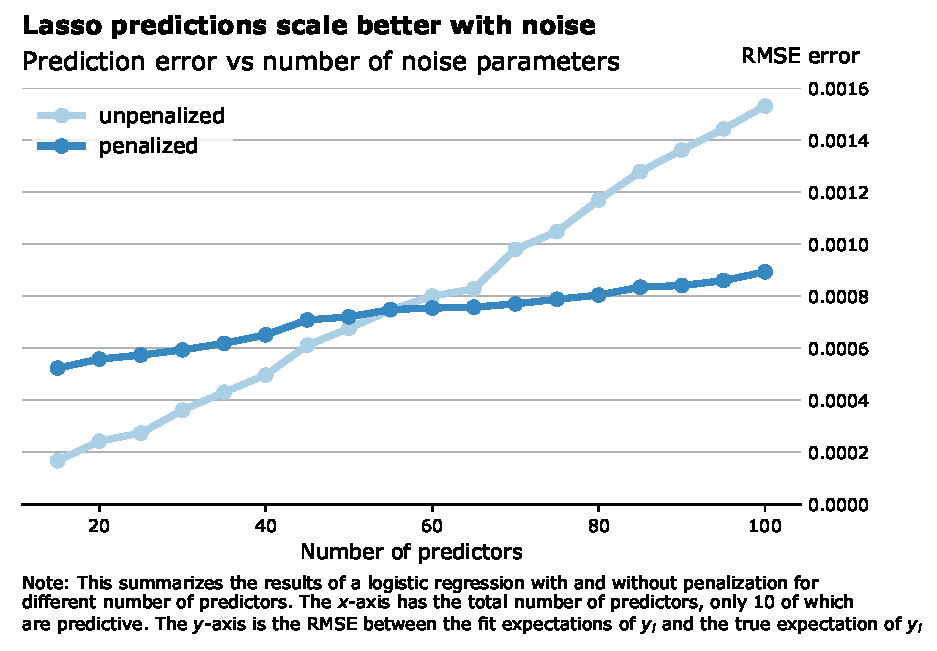
\includegraphics[width=.8\textwidth]{figs/lasso-pred-error}
\caption{Lasso prediction error}
\label{fig:lasso-pred-err}
\end{figure}

We can repeat this process for different values of $p$ keeping the number of
significant coefficients constant. This captures the insertion of noisy
parameters into our problem. Then, we can plot the summary statistics against
the number of predictors both for our lasso solution as well as a standard
un-penalized logistic regression. \cref{fig:lasso-pred-err} shows us that while
the insertion of covariates with no predictive ability hurts our predictive
power in both the lasso and un-penalized cases, the lasso scales better as
evidenced by a smaller slope. Of course, the trade-off is that the un-penalized
solution does better in cases where more of the parameters are predictive ($p$
is smaller). In our particular experiment, the break-even point is at around 50
covariates for our chosen value of $\lambda$.

\begin{figure}[tbh]
\centering
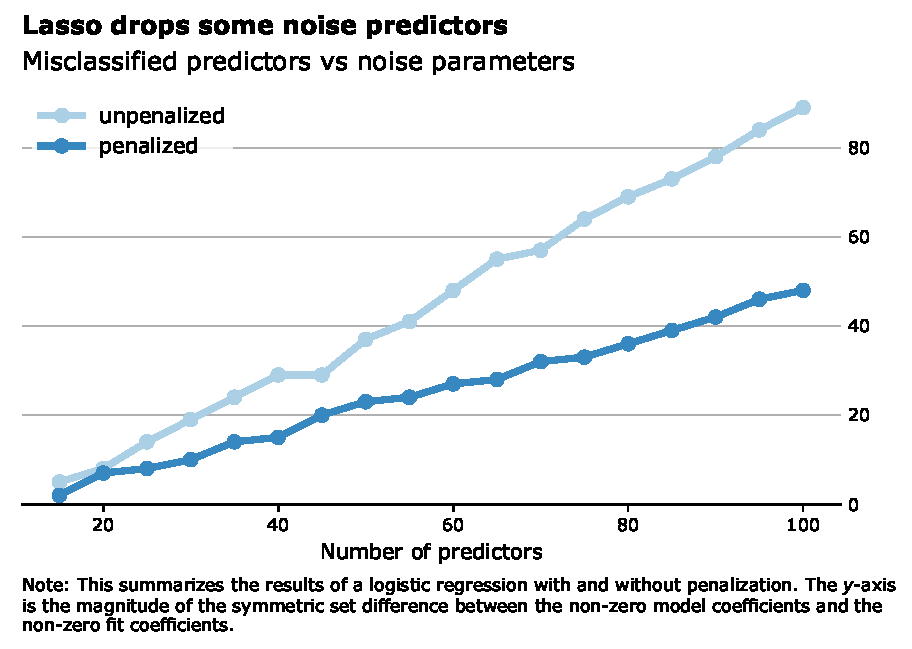
\includegraphics[width=.8\textwidth]{figs/lasso-symm-diff}
\caption{Lasso sparsity identification}
\label{fig:lasso-symm-diff}
\end{figure}

\begin{figure}[tb]
\centering
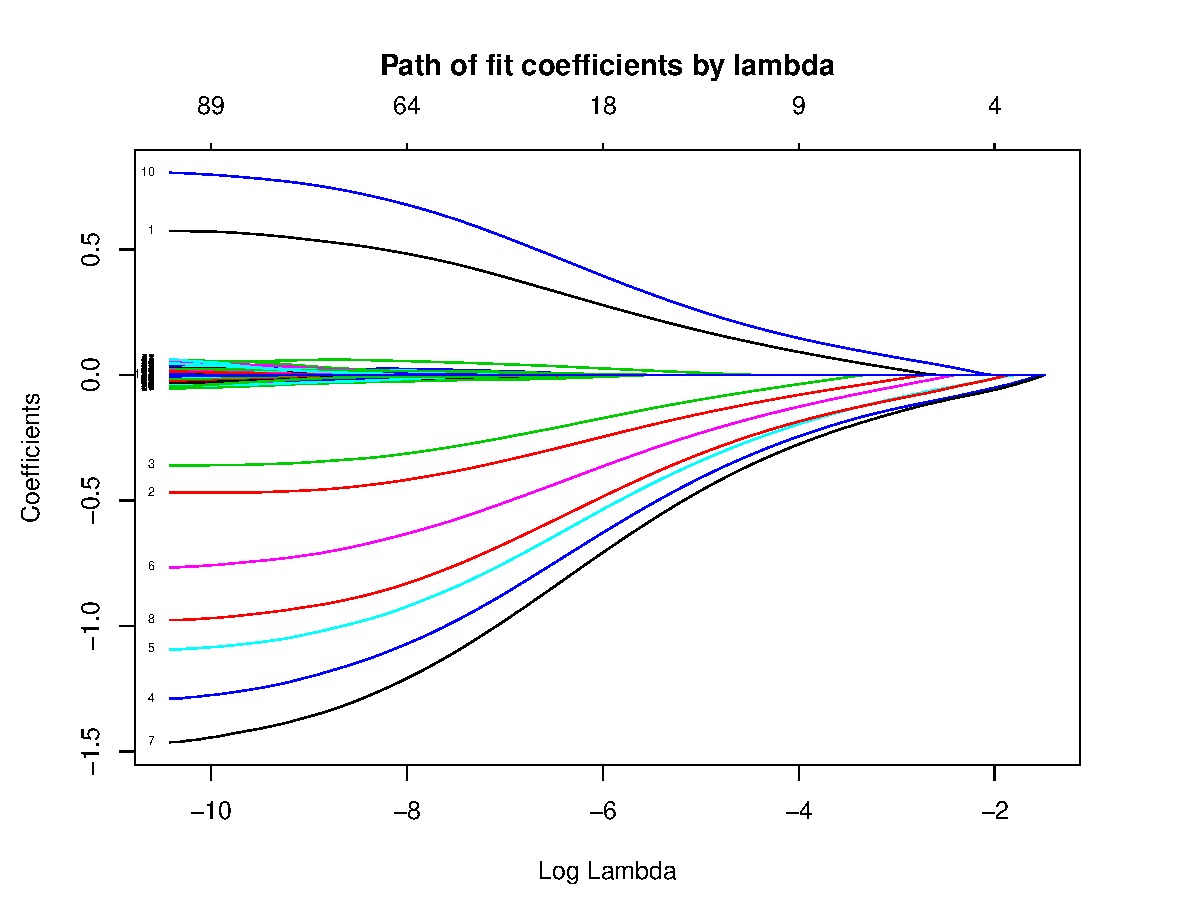
\includegraphics[width=.8\textwidth]{figs/lasso-path}
\caption{Lasso coefficient path}
\label{fig:lasso-path}
\end{figure}

We can also understand the implications of the lasso versus the un-penalized GLM
for model selection through \cref{fig:lasso-symm-diff}. This shows us that the
un-penalized GLM ascribes non-zero (which we here define as bigger in absolute
value than $10^{-3}$) coefficients to almost all the covariates, even when the
true coefficient for most of them is 0. The lasso with our chosen value of
$\lambda$ brings this value down to just about half. More sparsity can be
achieved by using a bigger $\lambda$, though this can also affect the predictive
loss.


Finally, we can also vary the adaptive parameter $\lambda$ and explore the
behavior of the coefficients as we do so. \cref{fig:lasso-path} uses R's
\textsf{glmnet} package to generate the plot of log $\lambda$ versus the
coefficients in the same model as previously. This illustrates the power of the
lasso for model selection: the coefficients of the non-predictive terms get
brought down to zero distinctly before that of the predictive term (the first 10
terms are predictive, and are labelled on the chart).

\section{Discussion and Conclusion}
\label{sec:conc}
In this report, we introduce the problem of high-dimensional regression in a
linear and generalized linear models context. We show that lasso has good
in-sample error and selection properties for the linear regression case, and we
state generalizations ofthe linear regression case in \Cref{sec:model}. We
introduced a few algorithms to compute the lasso in \Cref{sec:estimation},
including extensions to stochastic gradient and coordinate descent methods. We
 add numerical experiments to explore the behavior of the lasso in a sparse GLM
 setting in \Cref{sec:num}.  %\lipsum% [3]
\newpage
% \nocite{*}
\bibliographystyle{jpe}
\bibliography{sources}

\newpage

\section*{Appendix A: Code}

\begin{lstlisting}
import scipy

from scipy.special import expit

from sklearn.linear_model import LogisticRegression
from sklearn.metrics import mean_squared_error, 

n, p = int(1e5), 100
num_significant = 10

A = np.random.uniform(-1, 1, size=(p,p))
cov = A.T @ A
X = np.random.multivariate_normal(np.zeros(p), cov, n)
beta = np.zeros(p)
beta[:num_significant] = np.random.normal(size=num_significant)
y = np.random.binomial(1, expit(X @ beta)).astype(float)

logistic = LogisticRegression(penalty='l1', C=.1)

logistic.fit(X, y)
fit_coeffs = logistic.coef_.flatten()

mean_squared_error(expit(X @ beta), expit(X @ fit_coeffs))

len(set(range(num_significant)) ^ 
    set([i for i, val in enumerate(fit_coeffs) if abs(val) > 1e-3]))
\end{lstlisting}

\begin{lstlisting}
library(MASS)
library(psych)
library(glmnet)

# generate hyperparameters

n <- 1e4
p <- 100
num.significant <- 10

A <- matrix(runif(p^2)*2-1, ncol=p) 
sigma <- t(A) %*% A

# generate random data

X <- mvrnorm(n = n, Sigma = sigma, mu = rep(0, p))
beta <- rep(0, p)
beta[1:num.significant] = rnorm(num.significant)
eta <- as.vector(X %*% beta)

y <- as.numeric(runif(n) < logistic(eta))

# put together into a dataframe
# df <- as.data.frame(cbind(X, y))

l1.model <- glmnet(X, y, family = "binomial", alpha = 1)

plot.glmnet(l1.model, xvar = "lambda", label=TRUE)
title(main = "Path of fit coefficients by lambda", line = 2.5)
par(mar=c(4.5, 4.5, 5, 4))
\end{lstlisting}

\end{document}


